\section{}
Figure \ref{fig:Q3ProblemDiagram} shows a thin cantilever beam of unit thickness carrying a uniform load of intensity $p$ per unit length. 
Assume that the stress function is expressed by
\begin{equation*}
    \Phi = ax^2 + bx^2y + cy^3 + dy^5 + ex^2y^3
\end{equation*}
in which $a, ..., e$ are constants. Determine (a) the required values of $a, ..., e$ so that $\Phi$ is biharmonic;
(b) the stresses $\sigma_x$, $\sigma_y$, and $\tau_{xy}$
\begin{figure}[h]
    \centering
    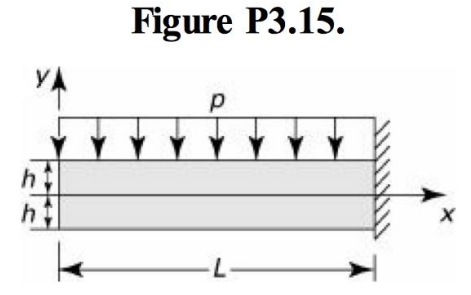
\includegraphics[width=0.3\linewidth]{Questions/Figures/Q3ProblemDiagram.png}
    \caption{Problem diagram for Question 3.}
    \label{fig:Q3ProblemDiagram}
\end{figure}

\subsection{}
The biharmonic equation is
\begin{equation*}
    \nabla^4 \Phi = \frac{\partial^4 \Phi}{\partial x^4} + 2 \frac{\partial^4 \Phi}{\partial x^2 \partial y^2} + \frac{\partial^4 \Phi}{\partial y^4} = 0
\end{equation*}
Substituting $\Phi$ into the biharmonic equation,
\begin{align*}
    \frac{\partial^4 \Phi}{\partial x^4} &= 0 \\
    \frac{\partial^4 \Phi}{\partial y^4} &= 120dy \\
    \frac{\partial^4 \Phi}{\partial x^2 \partial y^2} &= \frac{\partial^2}{\partial x^2} \left(6cy + 20dy^3 + 6ex^2y\right) = 12ey \\
    \implies \nabla^4 \Phi &= 0 + 2(12ey) + 120dy \overset{\text{set}}{=} 0 \\
    \implies e = -5d
\end{align*}
Therefore, $\Phi$ is biharmonic when $\boxed{e = -5d}$.

\subsection{}
The stress function can now be expressed as
\begin{equation*}
    \Phi = ax^2 + bx^2y + cy^3 + dy^5 - 5dx^2y^3 = ax^2 + bx^2y + cy^3 + d(y^5-5x^2y^3)
\end{equation*}
The boundary conditions are
\begin{align*}
    \tau_{xy}|_{y=\pm h} &= 0 \\
    \sigma_y|_{y=h} &= \frac{-pL}{Lt} = -\frac{p}{t} \\
    \sigma_y|_{y=-h} &= 0
\end{align*}
Since there is no axial load,
\begin{equation*}
    \int_{-h}^{h} \sigma_x y dy = 0
\end{equation*}
Finding expressions for $\sigma_x$, $\sigma_y$, and $\tau_{xy}$,
\begin{align*}
    \sigma_x &= \frac{\partial^2 \Phi}{\partial y^2} = 6cy + 20dy^2 - 30dx^2y \\
    \sigma_y &= -\frac{\partial^2 \Phi}{\partial x^2} = 2a + 2by - 10dy^3 \\
    \tau_{xy} &= -\frac{\partial^2 \Phi}{\partial x \partial y} = -2bx + 30dxy^2
\end{align*}
Applying the boundary conditions, first at $\tau_{xy}|_{y=h}$,
\begin{align*}
    \tau_{xy}|_{y=h} &= 0 \\
    \implies -2bx + 30dxh^2 &= 0 \\
    \implies b &= 15dh^2
\end{align*}
second at $\sigma_y|_{y=-h}$,
\begin{align*}
    \sigma_y|_{y=-h} &= 0 \\
    \implies 2a + 2(15dh^2)(-h) - 10d(-h)^3 &= 0 \\
    \implies a &= 10dh^3 
\end{align*}
lastly at $\sigma_y|_{y=h}$,
\begin{align*}
    \sigma_y|_{y=h} &= -\frac{p}{t} \\
    \implies 2(10dh^3) + 2(15dh^2)(h) - 10d(h)^3 &= -\frac{p}{t} \\
    \implies d &= \frac{p}{40h^3 t}
\end{align*}




